\clearpage
\subsection{Conclusioni}
Come si può osservare nei paragrafi \ref{sec:reticolo_confronto} e \ref{sec:prisma_confronto} le lunghezze d'onda calcolate combaciano qualitativamente con il colore delle righe spettrali osservate in entrambi gli esperimenti (reticolo e prisma).

\paragraph{Confronto spettro con metodo del reticolo e del prisma}
%
{Il metodo di diffrazione attrverso il reticolo risulta produrre meno bande, ma di maggiore intensità e più facilmente analizzabili dallo sperimentatore. Mentre, come detto nelle Conclusioni della sezione \ref{sec:prisma2}, il metodo del prisma presenta una maggiore imprecisione nel determinare l'esatta posizione di un singolo massimo in quanto se ne osservano molti a distanza ravvicinata.\\
Si ipotizza quindi che il metodo del reticolo sia più efficace per determinare lo spettro con tipologie di esperimenti simili a questo, con analisi da oculare di un telescopio per determinare la posizione dei massimi. Invece con metodi di analisi meno soggetti all'errore umano (si pensa ad esempio all'esposizione di una lastra fotografica) potrebbe essere più efficace il metodo del prisma in quanto rivela una maggior quantità di righe spettrali.}
%
% Spettro lampada C
%
    \begin{figure}[H]
    \centering
    \includegraphics[scale=0.8]{Grafici/O3_C_lampadaC_spectrum.eps}
    %\caption{}
    \label{fig:C3_P2_RL}
    \end{figure} 
%
% Spettro lampada D
    \begin{figure}[H]
    \centering
    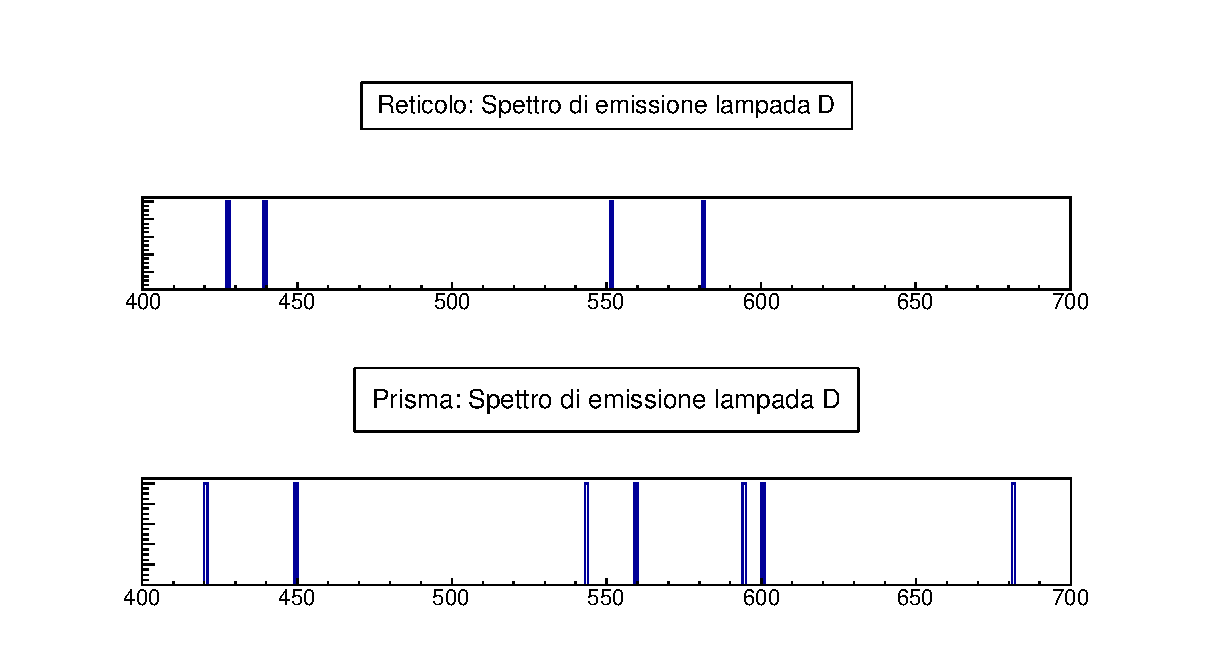
\includegraphics[scale=0.8]{Grafici/O3_C_lampadaD_spectrum.eps}
    %\caption{}
    \label{fig:C3_P2_RL}
    \end{figure} 
%
%
\paragraph{Identificazione materiali delle lampade}{
A causa dell'errore sperimentale troppo elevato, non si è riusciti a determinare con precisione gli elementi dal sito del NIST.}

\paragraph{Osservazioni aggiuntive}
\begin{itemize}
    \item Per poter utilizzare l’approssimazione di onda piana si deve realizzare una condizione di illuminazione corrispondente a una sorgente virtuale posta all’infinito. In tal modo è possibile considerare paralleli tutti i raggi uscenti dalla fenditura e porre la differenza di cammino ottico pari a $k d \sin\theta $
    \item Utilizzando questo spettrometro, si è previsto di riuscire a vedere circa 2 o 3 massimi a seconda della lunghezza d’onda.
    $$\sin\theta = n\frac{\lambda}{d} < 1 \Rightarrow n < \frac{d}{\lambda} \approx 3 $$
    Se ne osservano solamente 2, si ipotizza a causa delle condizioni di illuminazione della stanza.
    \item Il potere risolutivo del reticolo è $\frac{1}{nN}$, dove $N$ è il numero di fenditure. Non esssendo stata misurata la lunghezza del reticolo, non si è in grado di calcolarlo perchè, quindi non è noto $N$.
    \item Se fosse stato utilizzato un reticolo con passo più stretto, siccome $\sin\theta = n \frac{\lambda}{d}$, diminuendo $d$ aumenta l’angolo in cui viene osservata la lunghezza d’onda. Quindi si può diminuire l’errore relativo sull’angolo con misure di angoli grandi anche per i primi massimi.    
\end{itemize}
